	\section{Características del conjunto de datos} \label{specs}
		
		\begin{enumerate}
			\item Son eventos obtenidos mediante todos los disparos.
			\item Energía entre  [1 EeV , 2 EeV)
			\item Rango de tiempo:
			\begin{itemize}
				\item[-] Inicial:1388577600 (Thursday, 1 January 2014 12:00:00 GMT)
				\item[-] Final: 1577880000  (Thursday, 1 January 2020 12:00:00 GMT)
			\end{itemize}
			\item Ángulo cenital $\theta < 60^o$
			\item 6T5
			\item $ib=1$ Bad period flag. Un valor de 1 indica un buen periodo
			\item Número de eventos: $1\,081\,844$
		\end{enumerate}


\section{Bineado de eventos}

Clasificando a los eventos mencionados en la sección \ref{specs} según el valor de la ascensión recta, obtenemos el siguiente gráfico: 
\begin{figure}[H]
	\centering
	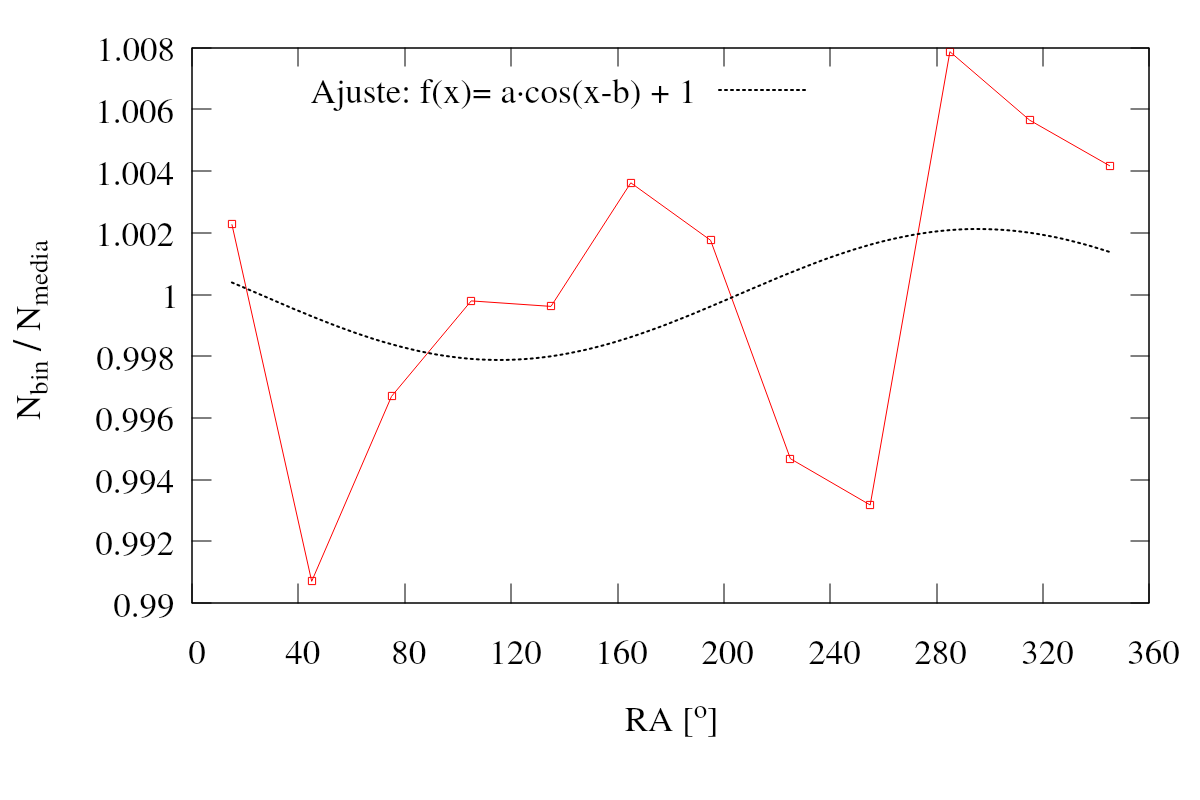
\includegraphics[width=0.95\textwidth]{bineado_eventos_herald_por_RA.png}
	\caption{me dejo}
\end{figure}

Si realizamos un ajuste de una función del tipo $f(x) = c\cdot(1 + a\cdot\cos{(\omega x - \phi)})$, se obtiene los siguientes valores
		
	Fase $\phi$ : $288(60)^o$  \\
	Amplitud $a$: 0.002(2) \footnote{Sí, el error es del 100\% para el ajuste.}  	 \\
		

\section{Pesos de los eventos}

			% Siderea:
			% 	Con la hora local: Le agregué 2 porque esa es la hora SIDEREA del cenit, así están en fase.
			% 	Con la ascensión recta:
		
		Para solucionar el desfase entre los pesos que obtengo mediante la hora local y la ascensión recta, lo que hice fue poner adrede un valor de desfase cuando calculo el valor $h$, le agregue $2\,$hr. 
		
		\begin{figure}[H]
			\centering
			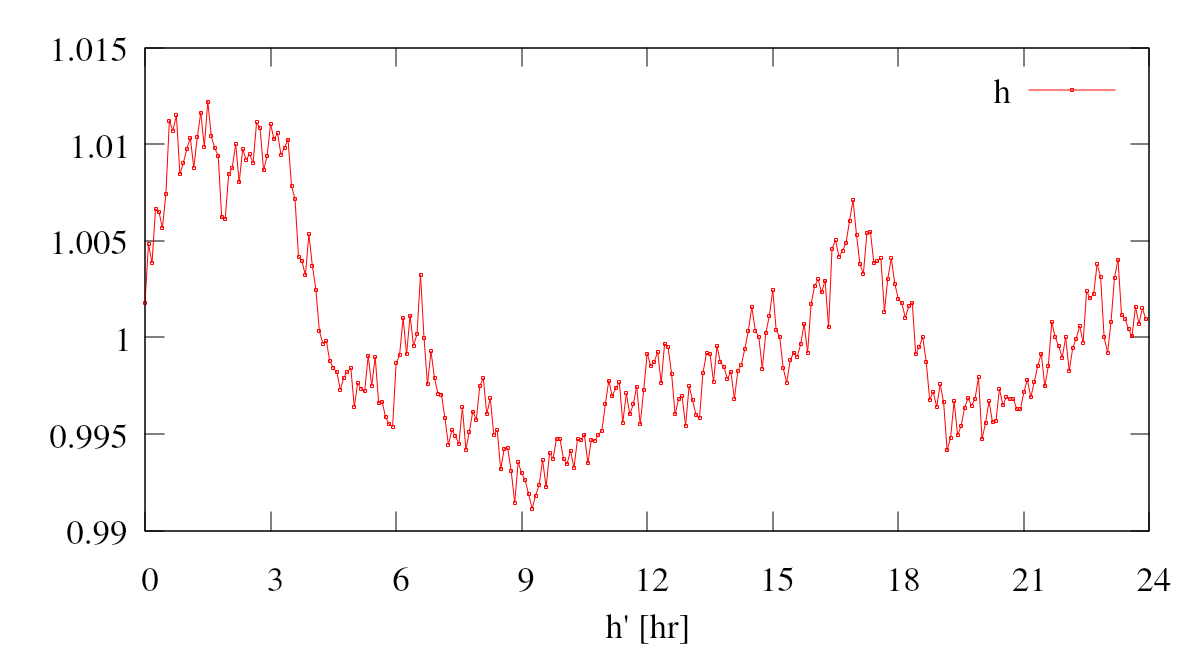
\includegraphics[width=0.65\textwidth]{eventos_hora_local.png}
			\caption{Usando el valor $h$ para calcular los pesos.}
		\end{figure}
		
		
		\begin{figure}[H]
			\centering
			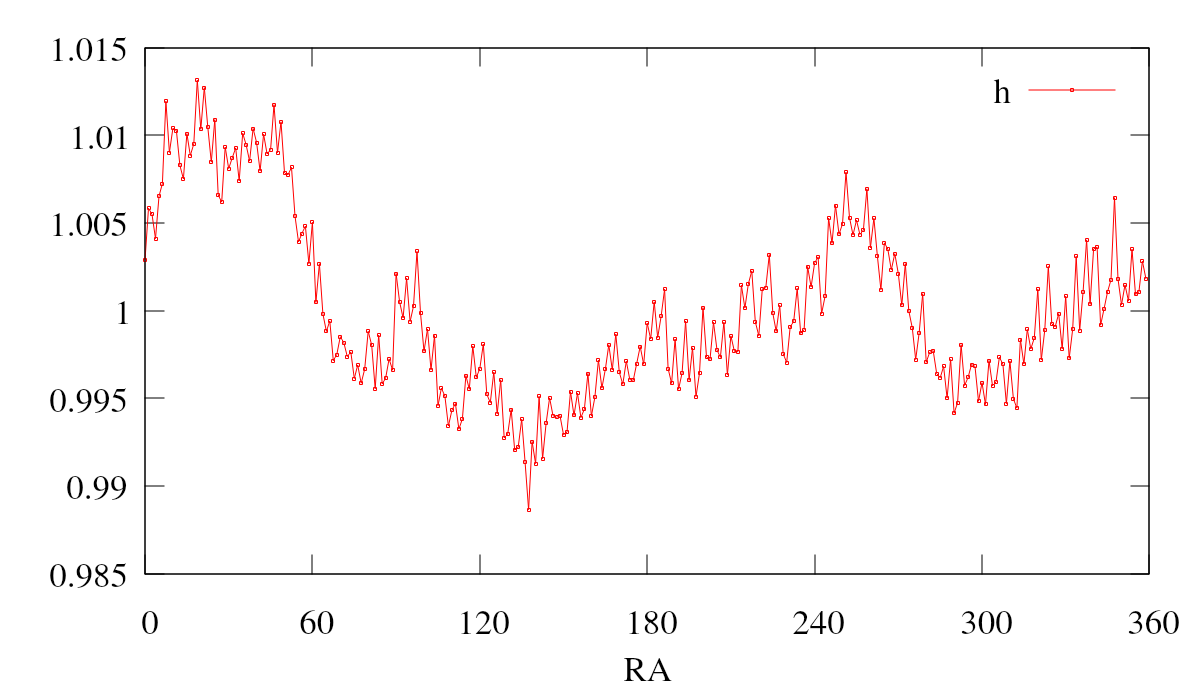
\includegraphics[width=0.65\textwidth]{eventos_RA.png}
			\caption{Usando la ascensión recta para calcular los pesos.}
		\end{figure}
		

\section{Grafico de la anisotropia}


		Lo de agregar un desfase adrede al valor de $h$ se puede hacer porque ya que para definir el valor del peso del evento, solo tiene que se debe ser consistente los valores  de h. Lo que no estoy teniendo en cuenta al hacer esta afirmación es que es cuando calculo la coordenada angular sobre la que hago el analisis en frecuencia
		\begin{equation}
			   \tilde{\alpha}_i = 2\pi \frac{h}{24} + \alpha_i -\alpha_{cenit,i},
		\end{equation}
		tiene en cuenta el valor de h. Probe en cambiar este desfase de $2\,$hr a otros valores arbitrarios para ver que pasaba. Lo que obtuve fue que la amplitud $r$ en el analisis de anisotropia se mantiene igual, pero la fase cambia. Los valores que muestro a continuación son dejando el desfase de h como $2\,$hr.
		
	\subsubsection{Tabla comparando:}
		
		\begin{table}[H]
		\centering
		
		\begin{tabular}{c|c|c}
					& Solar 		& Siderea\\ \hline
		Fase $\phi$ & 30(7) 	    & 356(5) 			\\
		Amplitud $a$& 0.0047(6)	    &0.0038(6)			\\
		\end{tabular}
		\caption{tabla}
		\end{table}
		
		
		
		\begin{figure}[H]
			\centering
			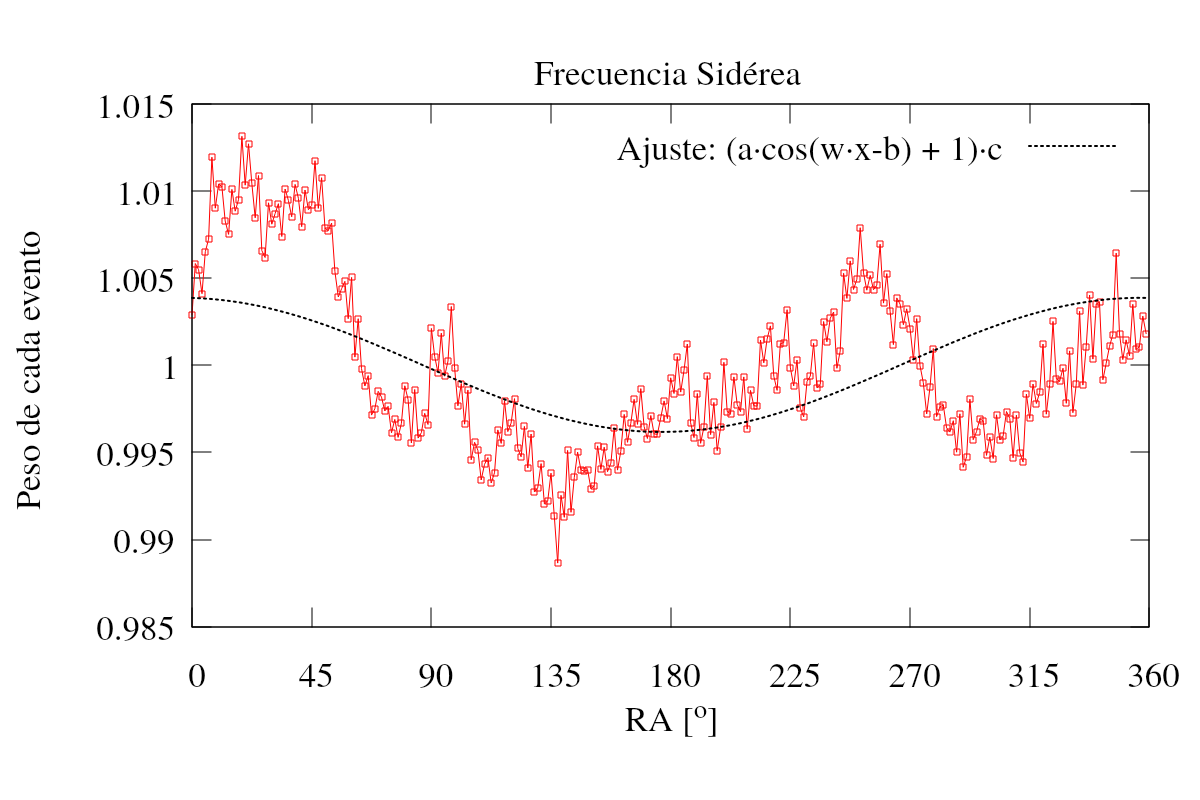
\includegraphics[width=0.95\textwidth]{eventos_RA_ajuste_cos.png}
			\caption{El ajuste hecho a la frecuencia sidérea usando el valor de $h$ para clasificar.}
		\end{figure}
		
		
		
		\begin{figure}[H]
			\centering
			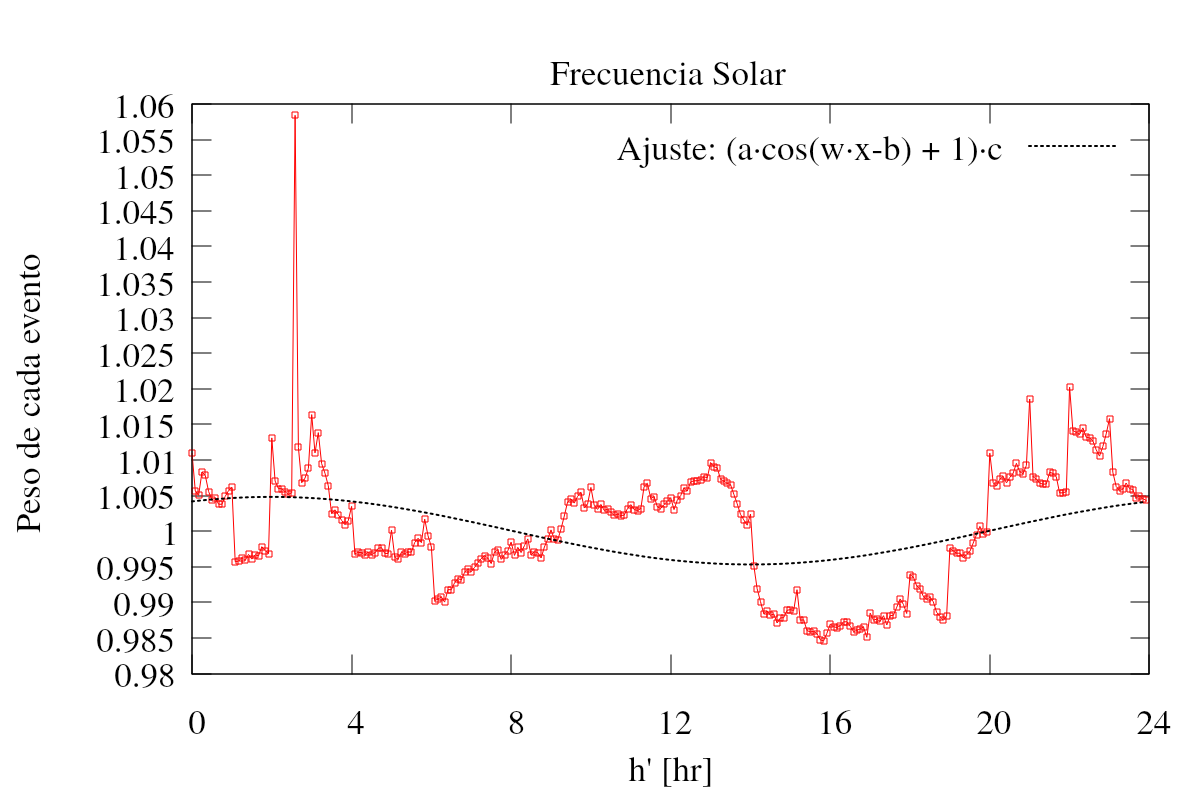
\includegraphics[width=0.95\textwidth]{eventos_hora_local_ajuste_cos.png}
			\caption{El ajuste hecho a la frecuencia sidérea usando el valor de la ascensión recta para clasificar.}
		\end{figure}
		
	\subsubsection{Análisis de anisotropías en ascensión recta}
		
		\begin{figure}[H]
			\centering
			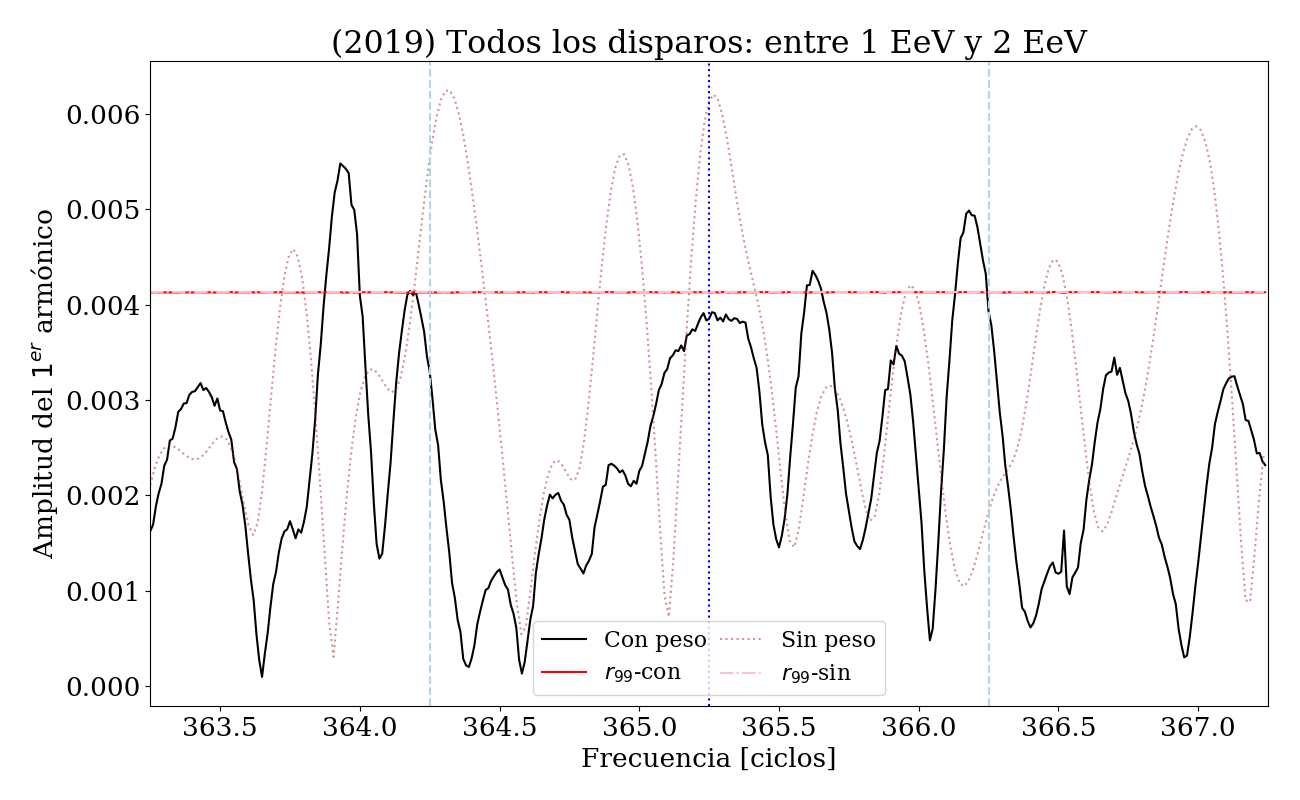
\includegraphics[width=0.95\textwidth]{pesos_sin_con_1_2_EeV.png}
			\caption{Anisotropía en función de la frecuencia, se comparan los análisis sin los pesos y con los pesos de los hexágonos}
		\end{figure}
		
		
		\begin{table}[H]
		\centering
		\begin{tabular}{c|c|c}
					& Solar (sin peso)		& Siderea (sin peso)  \\ \hline
		Fase $\phi$ & 224.681	    		& 335.104			\\
		Amplitud $r$& 0.00706339	    	&0.00404635			\\
		\end{tabular}
		\caption{TAbla}
		
		\end{table}
		
		\begin{table}[H]
		\centering
		\begin{tabular}{c|c|c}
					& Solar (con peso)		& Siderea (con peso)  \\ \hline
		Fase $\phi$ & 286.567	    	& 335.104			\\
		Amplitud $r$& 0.00383264	    &0.00404635			\\
		\end{tabular}
		\caption{TAbla}
		\end{table}
		
		
		